\documentclass{beamer} 
\usepackage{multicol}
\usepackage{url}
\usepackage{fancyvrb}
\usepackage{color}

\makeatletter
\def\PY@reset{\let\PY@it=\relax \let\PY@bf=\relax%
    \let\PY@ul=\relax \let\PY@tc=\relax%
    \let\PY@bc=\relax \let\PY@ff=\relax}
\def\PY@tok#1{\csname PY@tok@#1\endcsname}
\def\PY@toks#1+{\ifx\relax#1\empty\else%
    \PY@tok{#1}\expandafter\PY@toks\fi}
\def\PY@do#1{\PY@bc{\PY@tc{\PY@ul{%
    \PY@it{\PY@bf{\PY@ff{#1}}}}}}}
\def\PY#1#2{\PY@reset\PY@toks#1+\relax+\PY@do{#2}}

\def\PY@tok@gd{\def\PY@tc##1{\textcolor[rgb]{0.63,0.00,0.00}{##1}}}
\def\PY@tok@gu{\let\PY@bf=\textbf\def\PY@tc##1{\textcolor[rgb]{0.50,0.00,0.50}{##1}}}
\def\PY@tok@gt{\def\PY@tc##1{\textcolor[rgb]{0.00,0.25,0.82}{##1}}}
\def\PY@tok@gs{\let\PY@bf=\textbf}
\def\PY@tok@gr{\def\PY@tc##1{\textcolor[rgb]{1.00,0.00,0.00}{##1}}}
\def\PY@tok@cm{\let\PY@it=\textit\def\PY@tc##1{\textcolor[rgb]{0.25,0.50,0.50}{##1}}}
\def\PY@tok@vg{\def\PY@tc##1{\textcolor[rgb]{0.10,0.09,0.49}{##1}}}
\def\PY@tok@m{\def\PY@tc##1{\textcolor[rgb]{0.40,0.40,0.40}{##1}}}
\def\PY@tok@mh{\def\PY@tc##1{\textcolor[rgb]{0.40,0.40,0.40}{##1}}}
\def\PY@tok@go{\def\PY@tc##1{\textcolor[rgb]{0.50,0.50,0.50}{##1}}}
\def\PY@tok@ge{\let\PY@it=\textit}
\def\PY@tok@vc{\def\PY@tc##1{\textcolor[rgb]{0.10,0.09,0.49}{##1}}}
\def\PY@tok@il{\def\PY@tc##1{\textcolor[rgb]{0.40,0.40,0.40}{##1}}}
\def\PY@tok@cs{\let\PY@it=\textit\def\PY@tc##1{\textcolor[rgb]{0.25,0.50,0.50}{##1}}}
\def\PY@tok@cp{\def\PY@tc##1{\textcolor[rgb]{0.74,0.48,0.00}{##1}}}
\def\PY@tok@gi{\def\PY@tc##1{\textcolor[rgb]{0.00,0.63,0.00}{##1}}}
\def\PY@tok@gh{\let\PY@bf=\textbf\def\PY@tc##1{\textcolor[rgb]{0.00,0.00,0.50}{##1}}}
\def\PY@tok@ni{\let\PY@bf=\textbf\def\PY@tc##1{\textcolor[rgb]{0.60,0.60,0.60}{##1}}}
\def\PY@tok@nl{\def\PY@tc##1{\textcolor[rgb]{0.63,0.63,0.00}{##1}}}
\def\PY@tok@nn{\let\PY@bf=\textbf\def\PY@tc##1{\textcolor[rgb]{0.00,0.00,1.00}{##1}}}
\def\PY@tok@no{\def\PY@tc##1{\textcolor[rgb]{0.53,0.00,0.00}{##1}}}
\def\PY@tok@na{\def\PY@tc##1{\textcolor[rgb]{0.49,0.56,0.16}{##1}}}
\def\PY@tok@nb{\def\PY@tc##1{\textcolor[rgb]{0.00,0.50,0.00}{##1}}}
\def\PY@tok@nc{\let\PY@bf=\textbf\def\PY@tc##1{\textcolor[rgb]{0.00,0.00,1.00}{##1}}}
\def\PY@tok@nd{\def\PY@tc##1{\textcolor[rgb]{0.67,0.13,1.00}{##1}}}
\def\PY@tok@ne{\let\PY@bf=\textbf\def\PY@tc##1{\textcolor[rgb]{0.82,0.25,0.23}{##1}}}
\def\PY@tok@nf{\def\PY@tc##1{\textcolor[rgb]{0.00,0.00,1.00}{##1}}}
\def\PY@tok@si{\let\PY@bf=\textbf\def\PY@tc##1{\textcolor[rgb]{0.73,0.40,0.53}{##1}}}
\def\PY@tok@s2{\def\PY@tc##1{\textcolor[rgb]{0.73,0.13,0.13}{##1}}}
\def\PY@tok@vi{\def\PY@tc##1{\textcolor[rgb]{0.10,0.09,0.49}{##1}}}
\def\PY@tok@nt{\let\PY@bf=\textbf\def\PY@tc##1{\textcolor[rgb]{0.00,0.50,0.00}{##1}}}
\def\PY@tok@nv{\def\PY@tc##1{\textcolor[rgb]{0.10,0.09,0.49}{##1}}}
\def\PY@tok@s1{\def\PY@tc##1{\textcolor[rgb]{0.73,0.13,0.13}{##1}}}
\def\PY@tok@sh{\def\PY@tc##1{\textcolor[rgb]{0.73,0.13,0.13}{##1}}}
\def\PY@tok@sc{\def\PY@tc##1{\textcolor[rgb]{0.73,0.13,0.13}{##1}}}
\def\PY@tok@sx{\def\PY@tc##1{\textcolor[rgb]{0.00,0.50,0.00}{##1}}}
\def\PY@tok@bp{\def\PY@tc##1{\textcolor[rgb]{0.00,0.50,0.00}{##1}}}
\def\PY@tok@c1{\let\PY@it=\textit\def\PY@tc##1{\textcolor[rgb]{0.25,0.50,0.50}{##1}}}
\def\PY@tok@kc{\let\PY@bf=\textbf\def\PY@tc##1{\textcolor[rgb]{0.00,0.50,0.00}{##1}}}
\def\PY@tok@c{\let\PY@it=\textit\def\PY@tc##1{\textcolor[rgb]{0.25,0.50,0.50}{##1}}}
\def\PY@tok@mf{\def\PY@tc##1{\textcolor[rgb]{0.40,0.40,0.40}{##1}}}
\def\PY@tok@err{\def\PY@bc##1{\fcolorbox[rgb]{1.00,0.00,0.00}{1,1,1}{##1}}}
\def\PY@tok@kd{\let\PY@bf=\textbf\def\PY@tc##1{\textcolor[rgb]{0.00,0.50,0.00}{##1}}}
\def\PY@tok@ss{\def\PY@tc##1{\textcolor[rgb]{0.10,0.09,0.49}{##1}}}
\def\PY@tok@sr{\def\PY@tc##1{\textcolor[rgb]{0.73,0.40,0.53}{##1}}}
\def\PY@tok@mo{\def\PY@tc##1{\textcolor[rgb]{0.40,0.40,0.40}{##1}}}
\def\PY@tok@kn{\let\PY@bf=\textbf\def\PY@tc##1{\textcolor[rgb]{0.00,0.50,0.00}{##1}}}
\def\PY@tok@mi{\def\PY@tc##1{\textcolor[rgb]{0.40,0.40,0.40}{##1}}}
\def\PY@tok@gp{\let\PY@bf=\textbf\def\PY@tc##1{\textcolor[rgb]{0.00,0.00,0.50}{##1}}}
\def\PY@tok@o{\def\PY@tc##1{\textcolor[rgb]{0.40,0.40,0.40}{##1}}}
\def\PY@tok@kr{\let\PY@bf=\textbf\def\PY@tc##1{\textcolor[rgb]{0.00,0.50,0.00}{##1}}}
\def\PY@tok@s{\def\PY@tc##1{\textcolor[rgb]{0.73,0.13,0.13}{##1}}}
\def\PY@tok@kp{\def\PY@tc##1{\textcolor[rgb]{0.00,0.50,0.00}{##1}}}
\def\PY@tok@w{\def\PY@tc##1{\textcolor[rgb]{0.73,0.73,0.73}{##1}}}
\def\PY@tok@kt{\def\PY@tc##1{\textcolor[rgb]{0.69,0.00,0.25}{##1}}}
\def\PY@tok@ow{\let\PY@bf=\textbf\def\PY@tc##1{\textcolor[rgb]{0.67,0.13,1.00}{##1}}}
\def\PY@tok@sb{\def\PY@tc##1{\textcolor[rgb]{0.73,0.13,0.13}{##1}}}
\def\PY@tok@k{\let\PY@bf=\textbf\def\PY@tc##1{\textcolor[rgb]{0.00,0.50,0.00}{##1}}}
\def\PY@tok@se{\let\PY@bf=\textbf\def\PY@tc##1{\textcolor[rgb]{0.73,0.40,0.13}{##1}}}
\def\PY@tok@sd{\let\PY@it=\textit\def\PY@tc##1{\textcolor[rgb]{0.73,0.13,0.13}{##1}}}

\def\PYZbs{\char`\\}
\def\PYZus{\char`\_}
\def\PYZob{\char`\{}
\def\PYZcb{\char`\}}
\def\PYZca{\char`\^}
\def\PYZsh{\char`\#}
\def\PYZpc{\char`\%}
\def\PYZdl{\char`\$}
\def\PYZti{\char`\~}
% for compatibility with earlier versions
\def\PYZat{@}
\def\PYZlb{[}
\def\PYZrb{]}
\makeatother


\title{(Non) Comprehensive Guide to C/C++ Source Code Quality} 
\author{Sergey Kishchenko} 
\date{March 25th, 2011} 
\usetheme{CambridgeUS}
\usecolortheme{seagull}
\institute{Quickoffice}
\begin{document}

\frame{\titlepage}
\begin{frame} 
\frametitle{Product quality and source code quality}
\begin{multicols}{2}
\center{Source code}

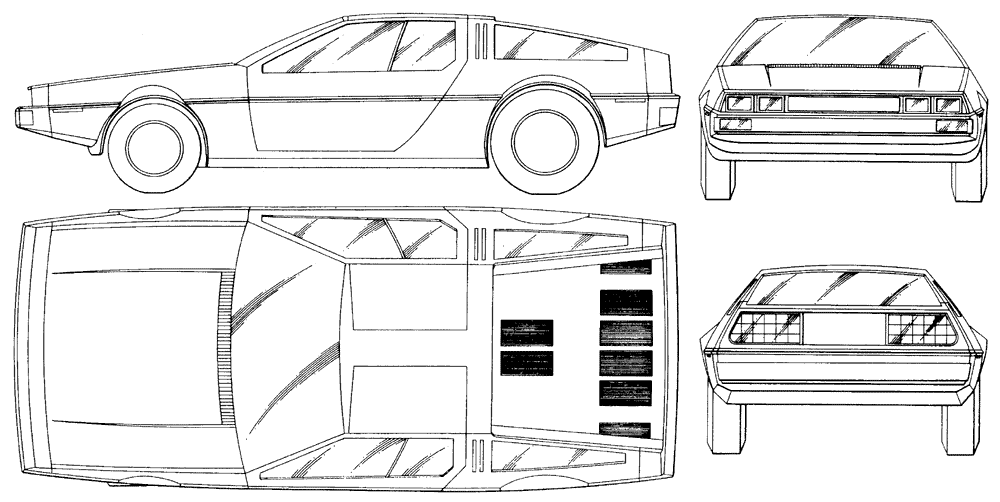
\includegraphics[width=0.4\textwidth]{img/delorean-blueprint}
\columnbreak
\center{Product}

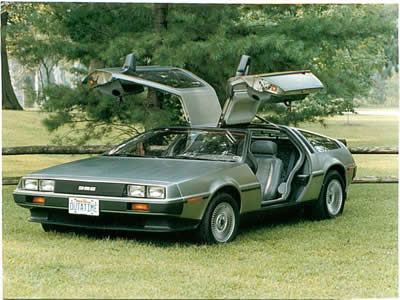
\includegraphics[width=0.4\textwidth]{img/delorean}
\end{multicols}
\begin{center}
\textbf{You can't make a good quality product with bad quality blueprint!}
\end{center}
\end{frame} 

\begin{frame}
\frametitle{Software product quality}
\begin{itemize}
\item Conformance to the specification
\item Completeness
\item Product documentation
\item \textbf{Source code quality}
\end{itemize}
\end{frame}

\begin{frame}
\frametitle{Source code quality}
\begin{itemize}
\item Correctness(no "bugs"!)
\item Maintainability
\item Readability
\item Portability
\item Low complexity
\item High code reuse
\item Efficiency
\end{itemize}
\end{frame}

\begin{frame}
\frametitle{Measuring source code quality}
\begin{itemize}
\item Bugs per line of code
\item Number of lines of code
\item Conformance to the code styling guide
\item Amount of platform-dependent code
\item Code coverage
\item Comment density
\item Program execution time, program size
\end{itemize}
\begin{center}
\textbf{There is no "silver bullet" source code quality metric :(}

\textbf{You should choose some of the points above and produce your own integral metric.}
\end{center}
\end{frame}

\begin{frame}
\begin{block}{\begin{center}\Large\textbf{How to measure and improve source code quality}\end{center}}
\begin{center}
\textbf{Part 1. Tools}
\end{center}
\end{block}
\end{frame}

\begin{frame}
\frametitle{CPD(Copy/Paste detection)}
\begin{center}
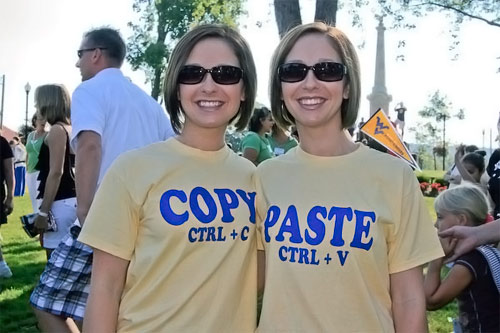
\includegraphics[width=0.4\textwidth]{img/copy-paste}
\end{center}
Improves readability, maintainability, increases code reuse, reduces resources usage. You can download it at \url{http://pmd.sourceforge.net/cpd.html}
\begin{exampleblock}{How to use}
java net.sourceforge.pmd.cpd.CPD --minimum-tokens 100 --files /path/to/cpp/source --language cpp
\end{exampleblock}
\end{frame}

\begin{frame}[fragile]
\frametitle{gcc -Wall -ansi -pedantic}
I'm serious, it is one of the best tools you can get. Do not underestimate it. Improves correctness and portability.
\begin{exampleblock}{How to use}
\begin{verbatim}
gcc -Wall -ansi -pedantic -c /path/to/source/file.cpp
\end{verbatim}
\end{exampleblock}
\end{frame}

\begin{frame}[fragile]
\frametitle{clang(static analizer)}
It's a C/C++/ObjC frontend for llvm. Improves correctness and portability. You can get clang at \url{http://clang.llvm.org/}
\begin{exampleblock}{How to use}
\begin{verbatim}
clang --analyze /path/to/source/file.cpp
\end{verbatim} 
\end{exampleblock}
\end{frame}

\begin{frame}[fragile]
\begin{exampleblock}{clang-test.cpp}
\begin{Verbatim}[commandchars=\\\{\}]
\PY{c+cp}{\PYZsh{}}\PY{c+cp}{include <stdio.h>}

\PY{k+kt}{int} \PY{n}{main}\PY{p}{(}\PY{k+kt}{int} \PY{n}{argc}\PY{p}{,} \PY{k+kt}{char}\PY{o}{*}\PY{o}{*} \PY{n}{argv}\PY{p}{)}
\PY{p}{\PYZob{}}
    \PY{k+kt}{char}\PY{o}{*} \PY{n}{fileName}\PY{p}{;} \PY{c+c1}{// not initialized!}
    \PY{k}{if} \PY{p}{(}\PY{l+m+mi}{2} \PY{o}{=}\PY{o}{=} \PY{n}{argc}\PY{p}{)}
    \PY{p}{\PYZob{}}
        \PY{n}{fileName} \PY{o}{=} \PY{n}{argv}\PY{p}{[}\PY{l+m+mi}{1}\PY{p}{]}\PY{p}{;}
    \PY{p}{\PYZcb{}}
    \PY{c+c1}{// using fileName}
    \PY{n}{FILE}\PY{o}{*} \PY{n}{f} \PY{o}{=} \PY{n}{fopen}\PY{p}{(}\PY{n}{fileName}\PY{p}{,} \PY{l+s}{"}\PY{l+s}{r}\PY{l+s}{"}\PY{p}{)}\PY{p}{;}
    \PY{n}{fclose}\PY{p}{(}\PY{n}{f}\PY{p}{)}\PY{p}{;}
\PY{p}{\PYZcb{}}
\end{Verbatim}
\end{exampleblock}
\end{frame}

\begin{frame}[fragile]
\begin{exampleblock}{Result}
\begin{Verbatim}
clang-test.cpp:11:15: warning: Pass-by-value argument in 
      function call is undefined
    FILE* f = fopen(fileName, "r");
              ^     ~~~~~~~~
1 warning generated.
\end{Verbatim}
\end{exampleblock}
\end{frame}

\begin{frame}
\frametitle{Valgrind}
\begin{center}

\includegraphics[width=0.6\textwidth]{img/valgrind}
\end{center}
Improves correctness, efficiency. You can get valgrind at \url{http://valgrind.org}
\end{frame}

\begin{frame}[fragile]
\frametitle{Valgrind. Memcheck}
\begin{exampleblock}{Usage}
\begin{verbatim}
valgrind --tool=memcheck /path/to/binary
\end{verbatim}
or
\begin{verbatim}
valgrind --leak-check=full /path/to/binary
\end{verbatim}
\end{exampleblock}
\end{frame}

\begin{frame}[fragile]
\begin{exampleblock}{memcheck-test.cpp}
\begin{Verbatim}[fontsize=\scriptsize,commandchars=\\\{\}]
\PY{c+cp}{\PYZsh{}}\PY{c+cp}{include <stdexcept>}
\PY{c+cp}{\PYZsh{}}\PY{c+cp}{include <iostream>}

\PY{k}{class} \PY{n+nc}{BuggyPool}
\PY{p}{\PYZob{}}
\PY{k}{public}\PY{o}{:}
    \PY{n}{BuggyPool}\PY{p}{(}\PY{k+kt}{int}\PY{o}{*} \PY{n}{data}\PY{p}{)}
    \PY{p}{\PYZob{}}
        \PY{k}{throw} \PY{n}{std}\PY{o}{:}\PY{o}{:}\PY{n}{runtime\PYZus{}error}\PY{p}{(}\PY{l+s}{"}\PY{l+s}{Hello from BuggyPool}\PY{l+s}{"}
                                 \PY{l+s}{"}\PY{l+s}{(I was written in tough times)}\PY{l+s}{"}\PY{p}{)}\PY{p}{;}
    \PY{p}{\PYZcb{}}
\PY{p}{\PYZcb{}}\PY{p}{;}

\PY{k+kt}{void} \PY{n}{foo}\PY{p}{(}\PY{p}{)}
\PY{p}{\PYZob{}}
    \PY{k+kt}{int}\PY{o}{*} \PY{n}{values} \PY{o}{=} \PY{k}{new} \PY{k+kt}{int}\PY{p}{[}\PY{l+m+mi}{1024}\PY{p}{]}\PY{p}{;}
    \PY{n}{BuggyPool} \PY{n}{pool}\PY{p}{(}\PY{n}{values}\PY{p}{)}\PY{p}{;}
    \PY{c+c1}{// pool is used somehow}
    \PY{k}{delete} \PY{p}{[}\PY{p}{]} \PY{n}{values}\PY{p}{;}
\PY{p}{\PYZcb{}}
\end{Verbatim}
\end{exampleblock}
\end{frame}

\begin{frame}[fragile]
\begin{exampleblock}{memcheck-test.cpp(main function)}
\begin{Verbatim}[fontsize=\footnotesize,commandchars=\\\{\}]
\PY{k+kt}{int} \PY{n}{main}\PY{p}{(}\PY{p}{)}
\PY{p}{\PYZob{}}
    \PY{k}{try}
    \PY{p}{\PYZob{}}
        \PY{n}{foo}\PY{p}{(}\PY{p}{)}\PY{p}{;}
    \PY{p}{\PYZcb{}}
    \PY{k}{catch}\PY{p}{(}\PY{n}{std}\PY{o}{:}\PY{o}{:}\PY{n}{runtime\PYZus{}error}\PY{o}{&} \PY{n}{err}\PY{p}{)}
    \PY{p}{\PYZob{}}
        \PY{n}{std}\PY{o}{:}\PY{o}{:}\PY{n}{cout}\PY{o}{<}\PY{o}{<}\PY{l+s}{"}\PY{l+s}{ERROR: }\PY{l+s}{"}\PY{o}{<}\PY{o}{<} \PY{n}{err}\PY{p}{.}\PY{n}{what}\PY{p}{(}\PY{p}{)}\PY{o}{<}\PY{o}{<}\PY{n}{std}\PY{o}{:}\PY{o}{:}\PY{n}{endl}\PY{p}{;}
    \PY{p}{\PYZcb{}}
\PY{p}{\PYZcb{}}
\end{Verbatim}
\end{exampleblock}
\end{frame}

\begin{frame}[fragile]
\begin{exampleblock}{Result}
\begin{Verbatim}[fontsize=\footnotesize]
==8076== HEAP SUMMARY:
==8076==     in use at exit: 4,096 bytes in 1 blocks
==8076==   total heap usage: 3 allocs, 2 frees, 4,263 bytes allocated
==8076== 
==8076== 4,096 bytes in 1 blocks are definitely lost in loss record 1 of 1
==8076==    at 0x4025F0F: operator new[](unsigned int) (in /usr/lib/...)
==8076==    by 0x8048B55: foo() (memcheck-test.cpp:14)
==8076==    by 0x8048B8D: main (memcheck-test.cpp:24)
==8076== 
==8076== LEAK SUMMARY:
==8076==    definitely lost: 4,096 bytes in 1 blocks
==8076==    indirectly lost: 0 bytes in 0 blocks
==8076==      possibly lost: 0 bytes in 0 blocks
==8076==    still reachable: 0 bytes in 0 blocks
==8076==         suppressed: 0 bytes in 0 blocks
\end{Verbatim}
\end{exampleblock}
\end{frame}

\begin{frame}
\frametitle{cppcheck}
\begin{exampleblock}{How to use}
\end{exampleblock}
\end{frame}

\begin{frame}
\frametitle{avalanche}
\begin{exampleblock}{How to use}
\end{exampleblock}
\end{frame}

\begin{frame}
\frametitle{yasca}
\begin{exampleblock}{How to use}
\end{exampleblock}
\end{frame}

\begin{frame}
\begin{block}{\begin{center}\Large\textbf{How to measure and improve source code quality}\end{center}}
\begin{center}
\textbf{Part 2. General ideas}
\end{center}
\end{block}
\end{frame}

\begin{frame}
\frametitle{Code review}
Improves correctness, readability, maintainability
\begin{exampleblock}{How to use}
\end{exampleblock}
\end{frame}

\begin{frame}
\frametitle{Unit and functional tests}
\begin{exampleblock}{How to use}
\end{exampleblock}
\end{frame}

\begin{frame}
\frametitle{Tests coverage}
\begin{exampleblock}{How to use}
\end{exampleblock}
\end{frame}

\begin{frame}
\frametitle{frama-c}
\begin{exampleblock}{How to use}
\end{exampleblock}
\end{frame}

\begin{frame}
\frametitle{Continuous integration}
\begin{exampleblock}{How to use}
\end{exampleblock}
\end{frame}

\begin{frame}
\frametitle{doxygen}
\begin{exampleblock}{How to use}
\end{exampleblock}
\end{frame}

\end{document}
